\chapter{3D-фигуры}
% Preamble: \pgfplotsset{width=7cm,compat=1.18}
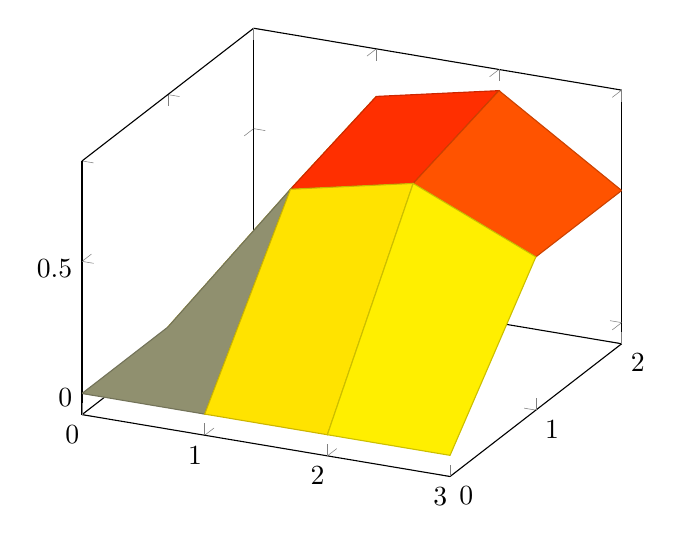
\begin{tikzpicture}
    \begin{axis}
        % this yields a 3x4 matrix:
        \addplot3 [surf] coordinates {
            (0,0,0) (1,0,0)   (2,0,0)   (3,0,0)
     
            (0,1,0) (1,1,0.6) (2,1,0.7) (3,1,0.5)
     
            (0,2,0) (1,2,0.7) (2,2,0.8) (3,2,0.5)
        };
    \end{axis}
    \end{tikzpicture}
    
% Preamble: \pgfplotsset{width=7cm,compat=1.18}
% requires \usepgfplotslibrary{colorbrewer}
\begin{tikzpicture}
    \begin{axis}[
        colormap/PuOr,
    ]
        \addplot3+ [
            mesh,
            scatter,
            samples=10,
            domain=0:1,
        ] {x*(1-x)*y*(1-y)};
    \end{axis}
    \end{tikzpicture}

% Preamble: \pgfplotsset{width=7cm,compat=1.18}
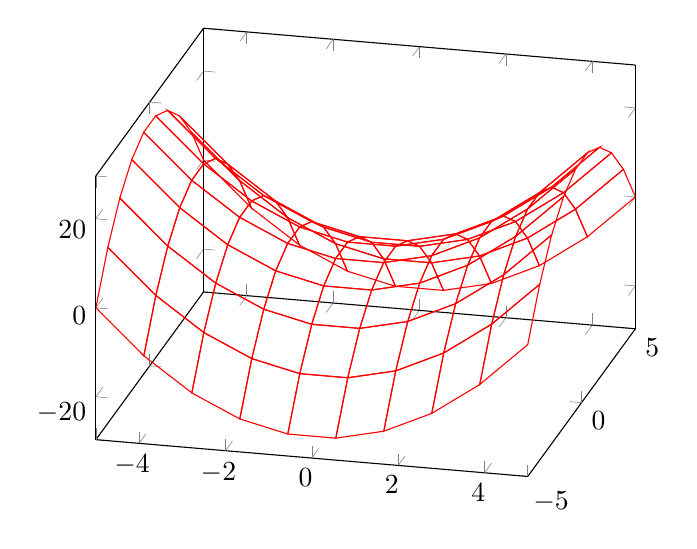
\begin{tikzpicture}
    \begin{axis}[view/az=14]
        \addplot3 [
            mesh,
            draw=red,
            samples=10,
        ] {x^2-y^2};
    \end{axis}
\end{tikzpicture}


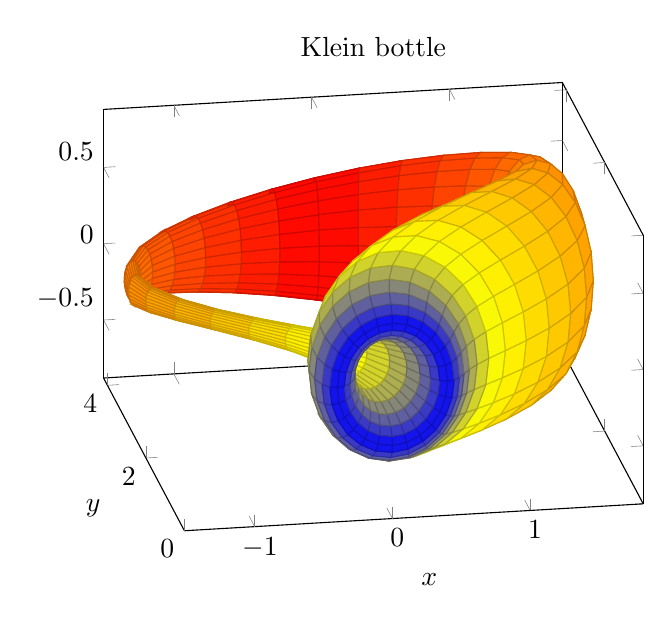
\begin{tikzpicture}
    \begin{axis}[
        xlabel=$x$, ylabel=$y$,
        view/h=-10,
        title=Klein bottle,
    ]
        \addplot3 [
            surf,
            z buffer=sort,
            colormap={periodic}{
                color=(blue)
                   color=(yellow)
                      color=(orange)
                         color=(red)
                      color=(orange)
                   color=(yellow)
                color=(blue)},
            domain=0:180, domain y=0:360,
            samples=41, samples y=25,
            variable=\u, variable y=\v,
            point meta=u,
        ] (
{-2/15 * cos(u) * (
3*cos(v) - 30*sin(u)
+ 90 *cos(u)^4 * sin(u)
- 60 *cos(u)^6 * sin(u)
+ 5 * cos(u)*cos(v) * sin(u))
},
{-1/15 * sin(u) * (3*cos(v)
- 3*cos(u)^2 * cos(v)
- 48 * cos(u)^4*cos(v)
+ 48*cos(u)^6 *cos(v)
- 60 *sin(u)
+ 5*cos(u)*cos(v)*sin(u)
- 5*cos(u)^3 * cos(v) *sin(u)
- 80*cos(u)^5 * cos(v)*sin(u)
+ 80*cos(u)^7 * cos(v) * sin(u))
},
{2/15 * (3 + 5*cos(u) *sin(u))*sin(v)}
);
    \end{axis}
\end{tikzpicture}


\begin{tikzpicture}
\begin{axis}[
        xlabel=$x$,
        ylabel=$y$,
        zlabel=$z$,
        title={Поверхность $z=x^2+y^2$},
        view={60}{30},  % Углы обзора
        grid=both,
        colormap/hot,
    ]
    \addplot3[
        surf,
        samples=50,
        domain=-2:2,
        y domain=-2:2,
    ]
    {x^2 + y^2};
\end{axis}
\end{tikzpicture}
